\chapter{Introduction}

Digital image alteration and manipulation have become ubiquitous issues in the current digital age,
fueling the spread of misinformation, deception, and even legal disputes. With the increasing
strength of artificial intelligence (AI), the creation of fake images has come to alarming levels,
making it increasingly difficult to distinguish between genuine and fake content. According
to a Google report \cite{yang2024}, AI-driven technologies such as generative adversarial
networks (GANs) and deepfake programs have contributed to an enormous hike in the creation of
fake images, thereby making broad-based misinformation on social media and other news channels
a reality. A highly high-profile case in point is the doctored image of an explosion in the Pentagon
\cite{pentagonExplosion}, which went viral and caused public panic before being discredited---this
is an example of the speed at which misinformation spreads.

\begin{figure}[htpb]
    \centering
    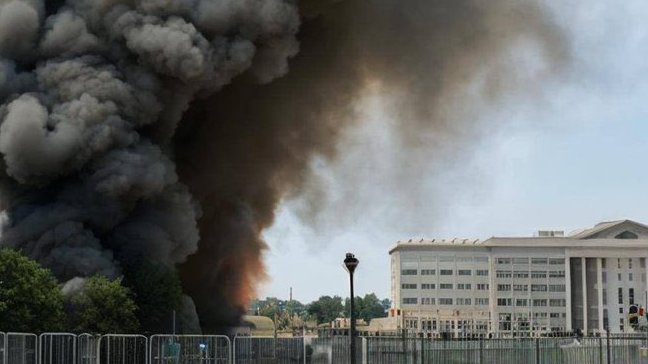
\includegraphics[width=0.8\textwidth]{images/fakePentagonImage.png}
    \caption{Fake image of the Pentagon explosion that went viral \cite{thetimesStockMarketImage}.}
    \label{fig:fakePentagonImage}
\end{figure}

Social networking sites have a key role to play in continuing this problem, as they offer fertile
ground for image manipulation. The ``Photoshop Epidemic'' \cite{photoshopEpidemic} demonstrates
how easily accessible image manipulation software can warp reality and compromise the integrity
of images. Even celebrities like Kate Middleton have been involved in photo manipulation scandals
to the point of questioning the authenticity of media circulated to the public \cite{kateMiddletonControversy}.
These events demonstrate a public skepticism of pictorial media increasing and emphasize the
importance of having strong mechanisms for guaranteeing image integrity and preventing manipulations.

Blockchain technology, developed in 2008 \cite{nakamoto2008}, has proved to be an effective way
to overcome such issues. Through the use of a decentralized and unalterable ledger, blockchain
makes it possible to have tamper-proof proof of digital images. In contrast to conventional storage
methods where data can be modified at will, blockchain-based applications derive cryptographic
hashes from photo metadata---e.g., timestamps, location, and device information---and write them
into an unchangeable ledger. Any tampering causes the hash match to break, thereby automatically
identifying the tampering. Smart contracts also mechanize this validation to ensure images remain
unchanged over their lifetime. Applications such as PHOTOCHAIN and Go-Sharing show how blockchain
can ensure photo integrity by making users the masters of ownership and distribution while
eliminating manipulation across a range of platforms.

Besides images, blockchain technology safeguards other valuable assets. In the professional and
academic world, certificates stored and validated on the blockchain avoid the lagginess in the
traditional validation of credentials, thus reducing cases of forgery and speeding up verification
processes. In the medical field, blockchain enables secure sharing of confidential medical images---MRIs
and X-rays---thus maintaining data integrity for proper diagnosis while maintaining patient
confidentiality. With an open, decentralized, and unalterable platform, blockchain has demonstrated
unparalleled diversity of application across different industries.

This work discusses the underlying contribution of blockchain technology, namely smart contracts and
cryptographic metadata hashing, to the provision of tamper-proofing settings for photographs, diplomas,
and medical reports. It explains actual applications, possible constraints---such as scalability,
latency, and regulation---and future research directions. By identifying the distinct attributes of
blockchain, this study endeavors to highlight its worth as a required guarantee of digital authenticity
during a time in which artificial intelligence makes it increasingly challenging to determine genuine
from fraudulent.

% References (sample; adapt as needed in your .bib file or a thebibliography environment)
% \begin{thebibliography}{9}
% \bibitem{googleReport} Author(s). (Year). Title of the Google report.
% \bibitem{pentagonExplosion} Author(s). (Year). Article/report on the Pentagon explosion hoax.
% \bibitem{photoshopEpidemic} Author(s). (Year). The "Photoshop Epidemic."
% \bibitem{kateMiddleton} Author(s). (Year). Article/report on Kate Middleton photo manipulation scandal.
% \bibitem{blockchain2008} Author(s). (2008). Original blockchain publication or reference.
% \end{thebibliography}
